\documentclass{article}
\usepackage{graphicx} % Required for inserting images
\usepackage[utf8]{inputenc}
\usepackage{polski}
\usepackage[dvipsnames]{xcolor}
\usepackage{indentfirst}
\usepackage{multicol}
\usepackage{geometry}
\usepackage{titlesec}
\usepackage[colorlinks=true, linkcolor=gray, urlcolor=blue, citecolor=green]{hyperref}
\usepackage{makecell}
\usepackage{float}
\usepackage[polish]{babel}
\usepackage[T1]{fontenc}
\usepackage[justification=centering]{caption}
\usepackage[utf8]{inputenc} 
\usepackage{subfig}
\usepackage{changepage}


\usepackage{mwe} % for 'example-image'
\usepackage{newfloat}
\DeclareFloatingEnvironment{graph}
\addto\captionspolish{%
  \renewcommand{\graphname}{Wykres}%
  \renewcommand{\figurename}{Zdjęcie}%
  \renewcommand{\tablename}{Tabela}%
}


\begin{document}

\begin{titlepage}
    \begin{center}
        \vspace*{1cm}
            
        \Huge
        \textbf{Sprawozdanie z laboratorium 3}
            
        \vspace{0.5cm}
        \LARGE
        Modbus 
            
        \vspace{1.5cm}
            
        \textbf{Łukasz Janusz\\Marek Generowicz}

        \normalsize      
        \textcolor{gray}{27.03.2025}
        \vfill
        \begin{figure}[hb]
            \centering
            
\includegraphics[width=0.5\textwidth]{media/Logo_AGH.jpg}
        \end{figure}   
    \end{center}
\end{titlepage}

\section{Wstęp}
Na zajęciach za zadanie mieliśmy zapoznać się z komunikacją Modbus RTU oraz stworzyć prosty program w języku drabinkowym, który będzie komunikował się z aplikacją \textit{ModRSsim2}.

Protokół Modbus jest popularnym protokołem komunikacyjnym, który jest szeroko stosowany w automatyce przemysłowej. Umożliwia on komunikację między urządzeniami, takimi jak sterowniki PLC, czujniki, napędy i inne urządzenia. Modbus RTU (Remote Terminal Unit) jest jedną z najczęściej używanych wersji tego protokołu, która wykorzystuje transmisję szeregową RS-232 lub RS-485.

Moduł ten oparty jest na architekturze slave-master, gdzie jedno urządzenie master może jednocześnie być podłączone do 247 urządzeń.

\begin{figure}[H]
    \centering
    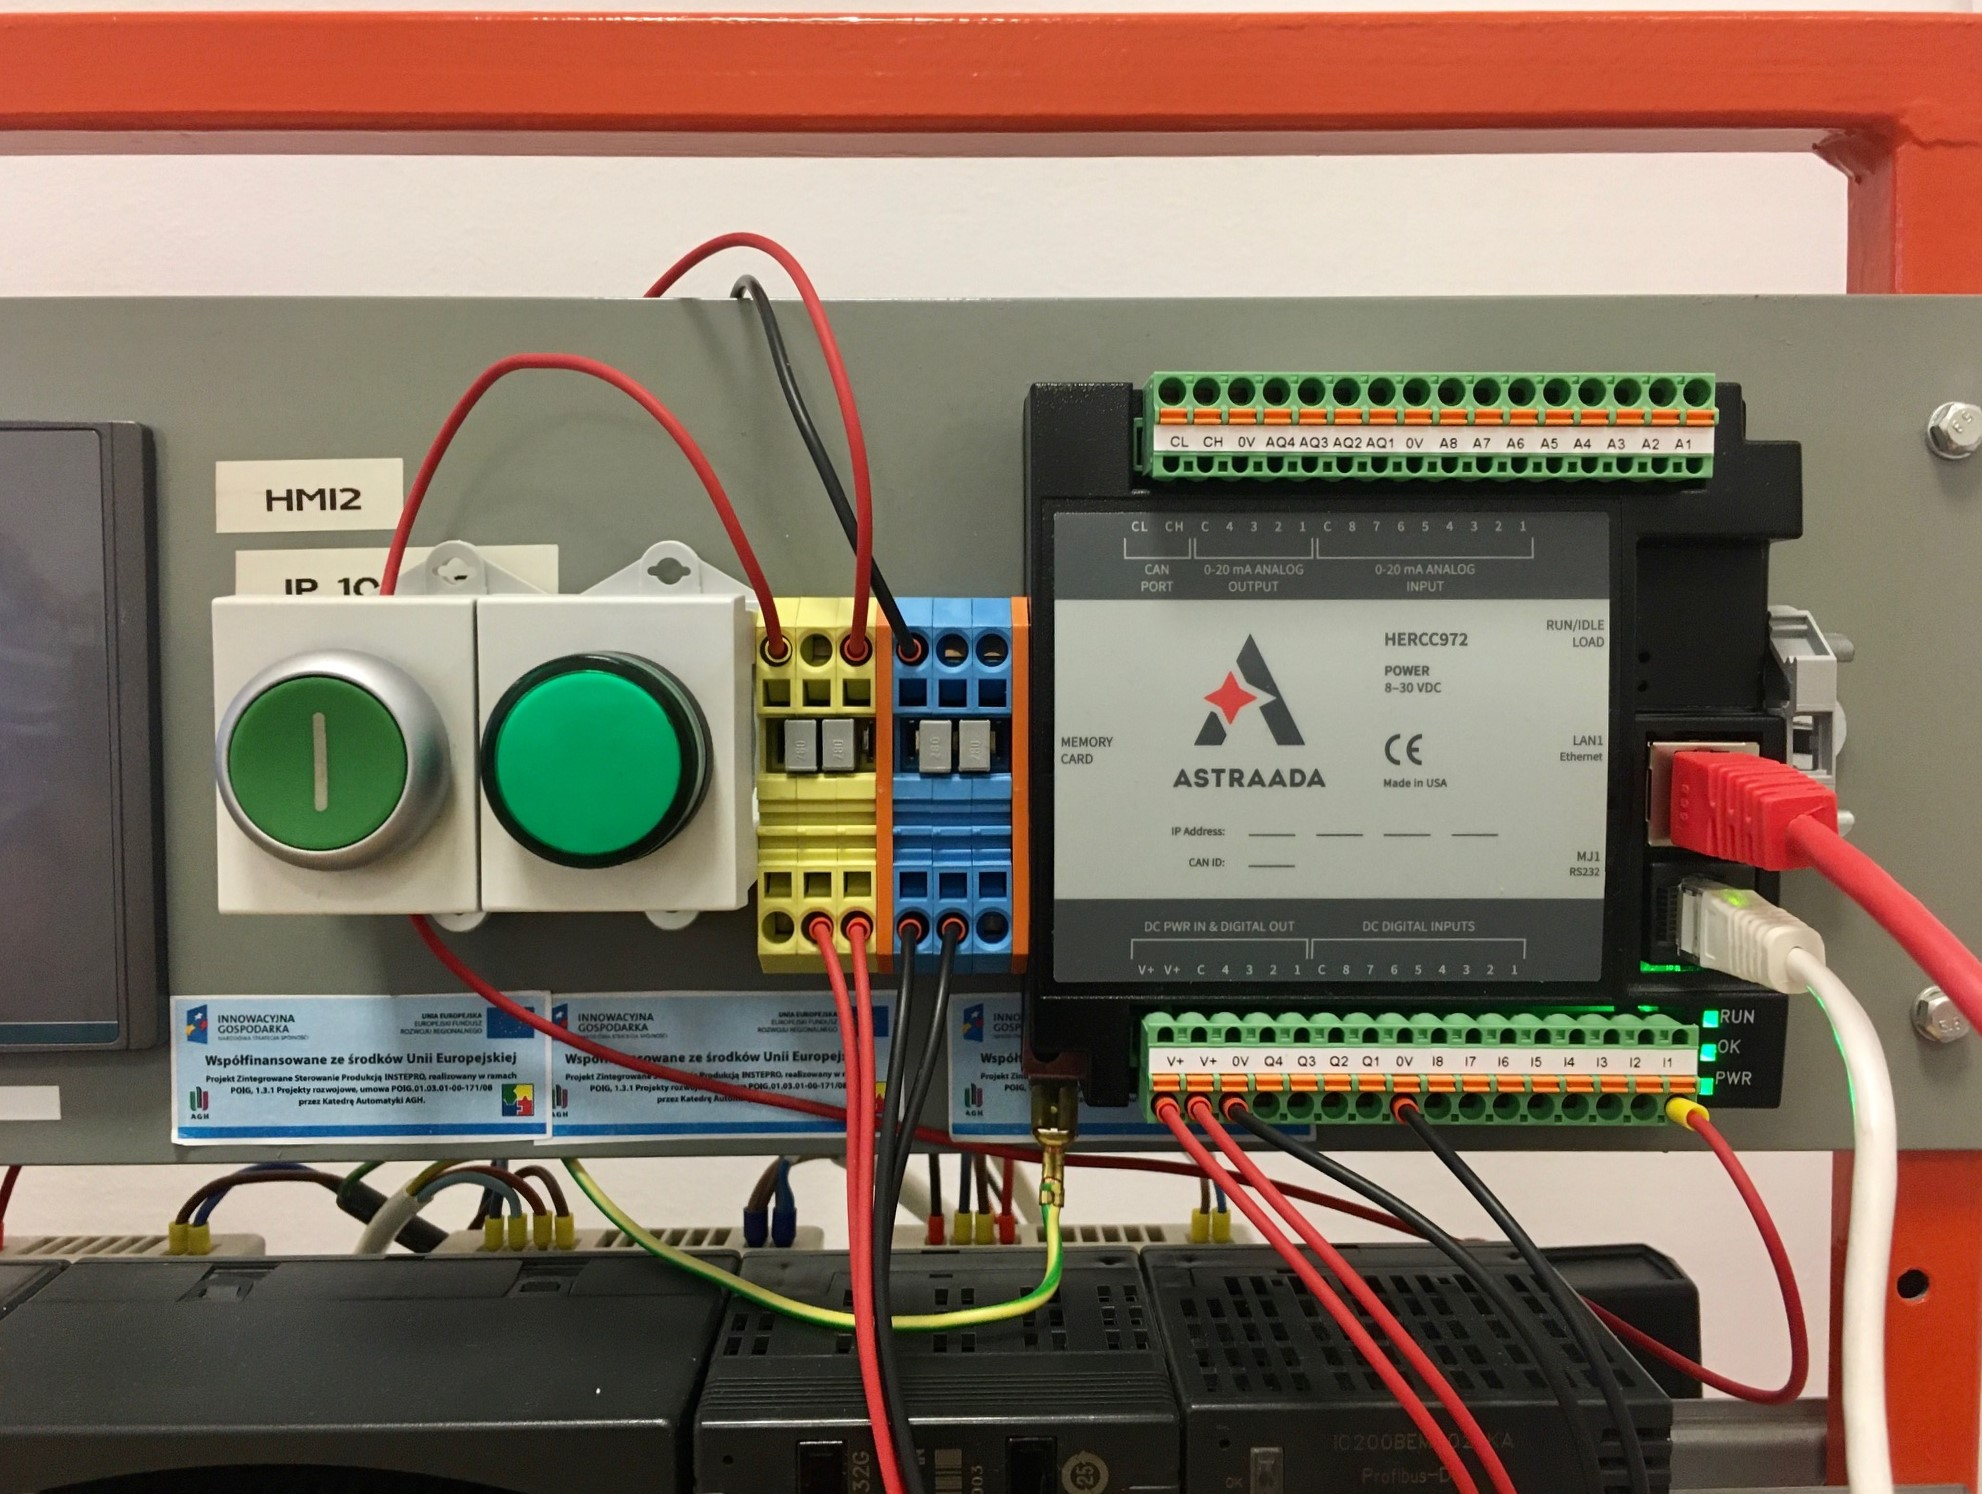
\includegraphics[width=0.92\textwidth]{media/0_stanowisko.jpg}
    \caption{Stanowisko laboratoryjne (zdjęcie z konspektu)}
    \label{fig:stanowisko}
\end{figure}


\newpage
\section{Przygotowanie projektu oraz programu w Cspace}


Przed przystąpieniem do ćwiczeń należało ustawić parametry sieciowe zgodnie z zdjęciem \ref{fig:zdj1} oraz potwierdzić konfiguracje za pomocą ethernetu wraz z podaniem poprawnego adresu IP, dzięki czemu możliwa jest komunikacja z PLC przez ethernet.
\begin{figure}[H]
    \centering
    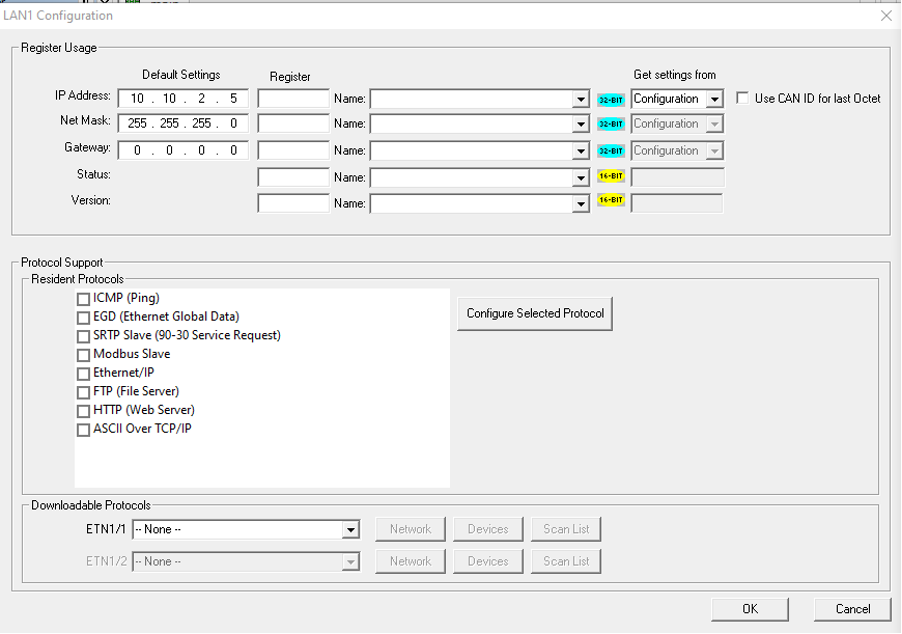
\includegraphics[width=0.5\textwidth]{media/4_0KonfiguracjaLan.png}
    \caption{Ustawienia parametrów LAN1 w Cspace}
    \label{fig:zdj1}
\end{figure}

Dzięki połączeniu z PLC w kolejnych krokach możliwe będzie przesyłanie kodu z komputera do PLC oraz odczyt i zapis danych z rejestrów Modbus. Ponieważ w PLC nadal znajduje się kod innej grupy, na dole ekranu widoczny jest parametr \textit{Not Equal}, tak jak na zdjęciu \ref{fig:zdj2}, co oznacza, że kod zapisany w PLC różni się od kodu w aplikacji.
\begin{figure}[H]
    \centering
    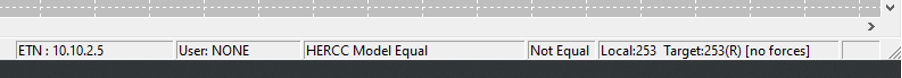
\includegraphics[width=0.5\textwidth]{media/4_1BezKody.png}
    \caption{Listwa statusu z niespójnym kodem w PLC}
    \label{fig:zdj2}
\end{figure}

\newpage
Następnie należało stworzyć prosty układ do zapalania diody kiedy guzik zostanie kliknięty oraz zgaszenia jej kiedy przestanie guzik nie będzie kliknięty. Na zdjęciu \ref{fig:zdj3} w listwie statusu widać również że kod został pomyślnie wgrany i zgadza się z tym co jest w PLC.

\begin{figure}[!ht]
    \centering
        % Pod figura 1
        \subfloat[Kod programu]{    
            \centering
            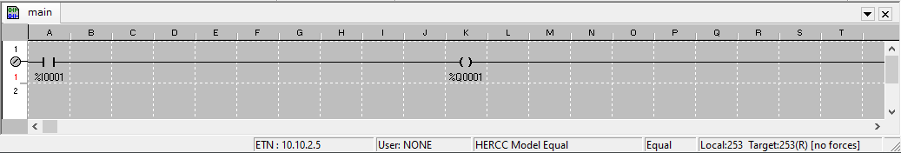
\includegraphics[width=0.5\textwidth]{media/4_2Zkodem.png}
            \label{fig:zdj3}}
        % Pod figura 2
        \subfloat[Debugowanie aktywnego układu]{
            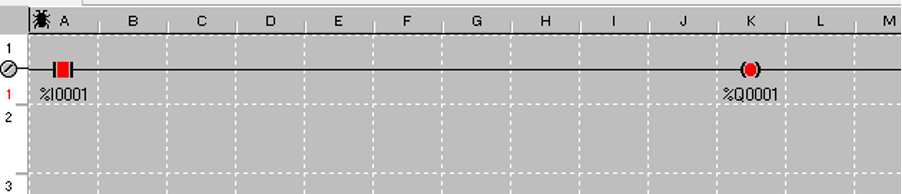
\includegraphics[width=0.5\textwidth]{media/4_3DebugON.png}            \label{fig:zdj4}
        }
   
        \hfill
     % Pod figura 1
    \subfloat[Rzeczywisty układ aktywny]{
        \includegraphics[width=0.5\textwidth]{media/4_5RzeczywistyprzyciskOFF.png}
        \label{fig:zdj5}}
    % Pod figura 2
    \subfloat[Rzeczywisty układ nieaktywny]{
        \includegraphics[width=0.5\textwidth]{media/4_4RzeczywistyprzyciskON.png}
        \label{fig:zdj6}
    }
    \caption{Konfiguracja kanałów modułu}
    \label{fig:main1}
\end{figure}


\newpage
\section{Obsługa oraz testy komunikacji}
Po pomyślnym wgraniu kodu należało przejść do stworzenia tagów komunikacyjnych ułatwiających komunikacje z Modbus. Każdy z tagów powinien być 16 bitowy. Na zdjęciu \ref{fig:zdj9} przedstawione jest jak należało zainicjować tagi oraz do czego każdy z nich był używany.


\begin{figure}[H]
    \centering
    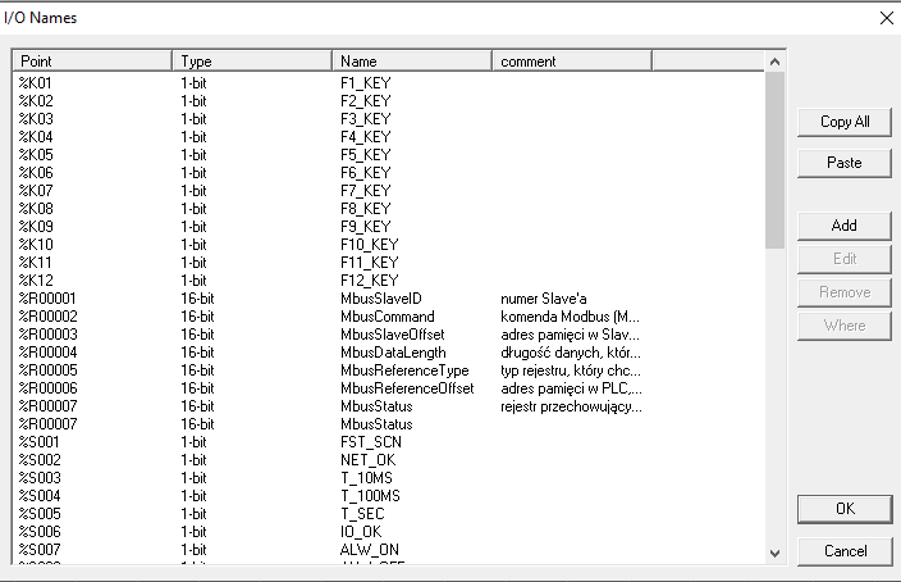
\includegraphics[width=0.5\textwidth]{media/5_3_IOnames.png}
    \caption{Tagi komunikacyjne}
    \label{fig:zdj9}
\end{figure}


Po utworzeniu tagów komunikacyjnych należało przejść do projektowania komunikacji z modułem Modbus dzięki czemu możliwe będzie odczytywanie i zapisywanie danych z rejestrów Modbus. W tym celu w Cspace należało aktywować komunikacje szeregową a następnie do  kodu należało dodać dwie drabinki kodu, zgodnie z zdjęciem \ref{fig:zdj7}.

Blok \textit{OPEN}na wyższej z drabinek służy do komunikacji z portem RS232, a moduł \textit{FST\_SCN} na tej drabince jest odpowiedzialny za jednokrotne działanie bloku. 

W niższej drabince moduł \textit{ALW\_ON} powoduje ciągłe działanie bloku \textit{MODBUS} który jest odpowiedzialny za obsługę protokołu Modbus Master. Zmienne przypisywane  do rejestrów Modbus są przypisane do tagów komunikacyjnych które zostały wcześniej utworzone.

\begin{figure}[H]
    \centering
    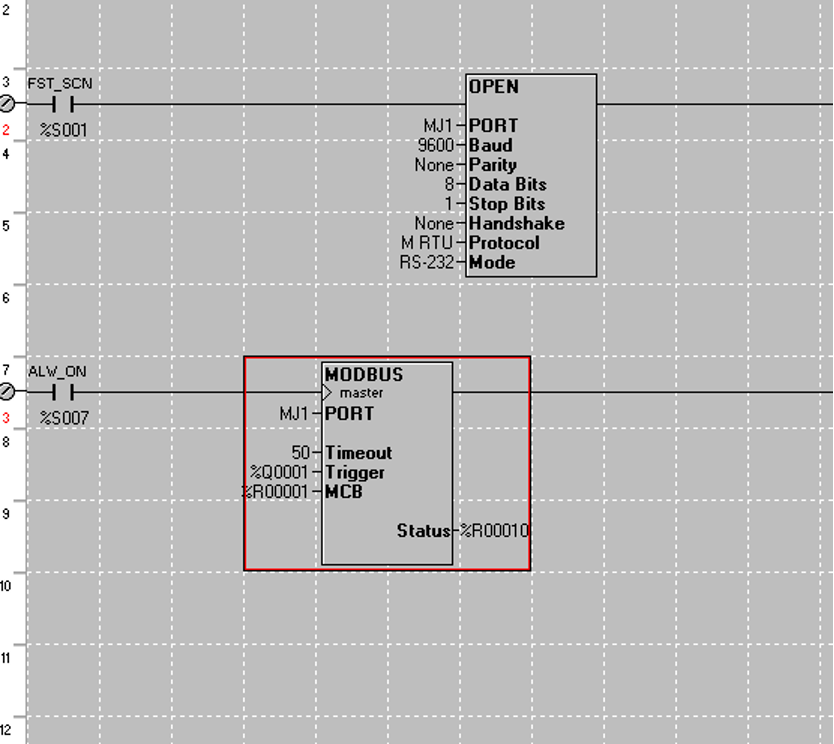
\includegraphics[width=0.5\textwidth]{media/5_1_Kolejnebloczki.png}
    \caption{Bloki do obsługi komunikacji z Modbus RTU}
    \label{fig:zdj7}
\end{figure}

% \begin{figure}[H]
%     \centering
%     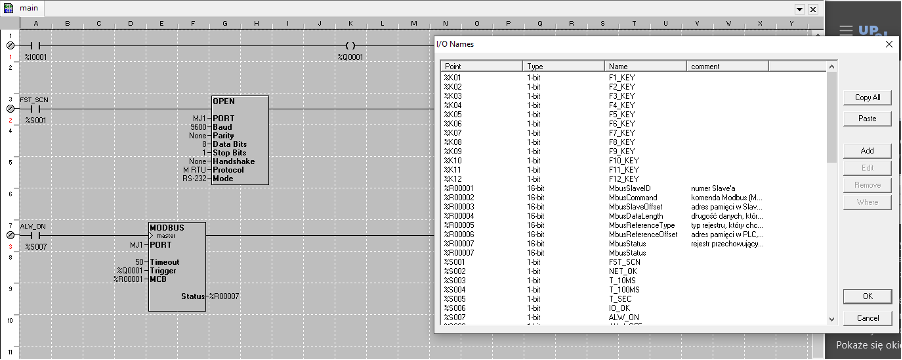
\includegraphics[width=0.5\textwidth]{media/5_2Kod&IOnames.png}
%     \caption{Stanowisko laboratoryjne (zdjęcie z konspektu)}
%     \label{fig:zdj8}
% \end{figure}

Przed przystąpieniem do testu należało również włączyć aplikacje \textit{ModRSsim2},
i skonfigurować go z portem do którego podłączony jest Modbus. Po tej operacji otrzymamy widok jak na zdjęciu \ref{fig:zdj10}. Aplikacja ta jest bardzo przydatna ponieważ pozwala nam na czytelny i widoczny odczyt danych wraz z ramkami komunikacyjnymi. Możliwe jest również ręczna zmiana danych w rejestrach Modbus.

\begin{figure}[H]
    \centering
    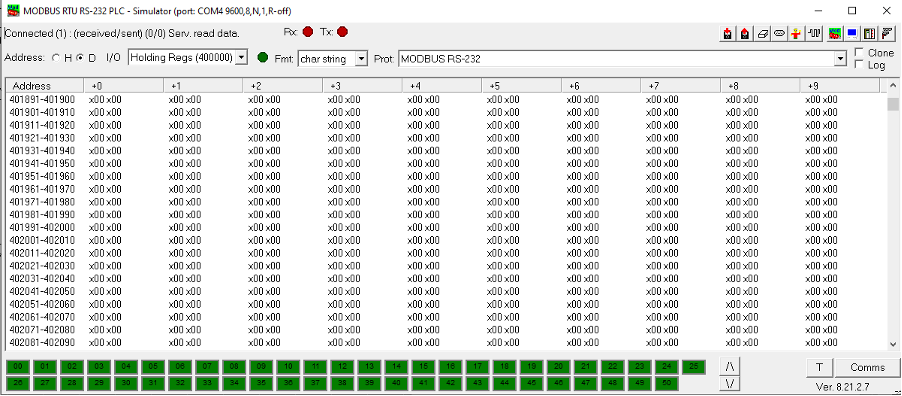
\includegraphics[width=0.5\textwidth]{media/5_4_Modbusapp.png}
    \caption{Widok rejestrów w aplikacji \textit{ModRSsim2}}
    \label{fig:zdj10}
\end{figure}

Po skonfigurowaniu komunikacji między aplikacją a PLC należało przejść do testów dzięki którym można było przetestować działanie oraz nauczyć się jak obsługiwać aplikacje.
\newpage
\subsection{Test 1}

W pierwszym teście należało umożliwić odczyt stanu pierwszej cewki ze Slave'a, należało ustawić parametry rejestru zgodnie z tabelą \ref{tab:tagi}. Dzięki takiemu ustawienie możliwe jest odczytanie stanu cewki. Aby to zrobić należało zmienić stan cewki w aplikacji \textit{ModRSsim2}. Aby odczytać stan cewki należało kliknąć przycisk na układzie tak jak na zdjęciu \ref{fig:zdj6}. W momencie kiedy cewka w aplikacji była ustawiona na 1, wartość zmiennej \textit{\%M00001} zmienił się z \texttt{OFF} na \texttt{ON}. Zdjęcie \ref{fig:zdj13} przedstawia zmianę stanu cewki zapisanej w zmiennej \textit{\%M00001} w aplikacji \textit{Cspace}.
% \begin{figure}[H]
%     \centering
%     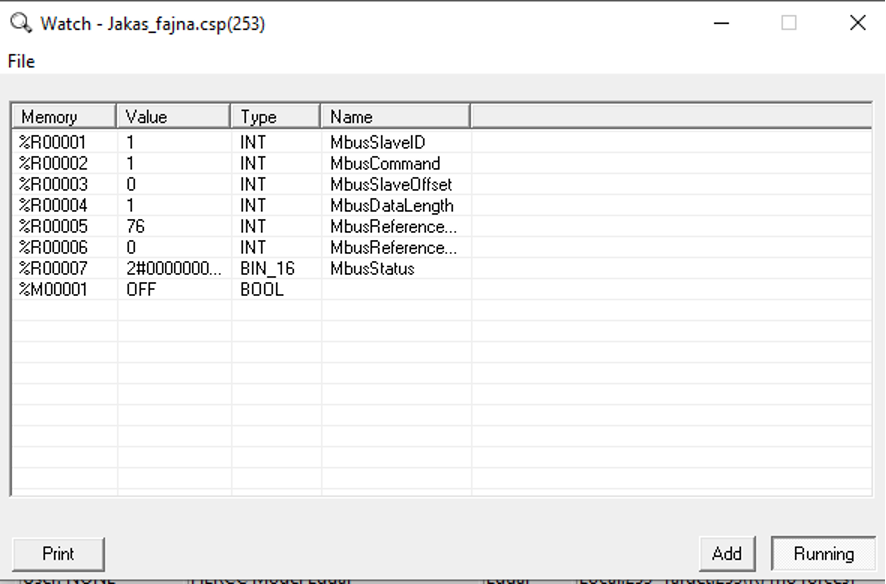
\includegraphics[width=0.5\textwidth]{media/5_test1_1_Watchzmienne.png}
%     \caption{Stanowisko laboratoryjne (zdjęcie z konspektu)}
%     \label{fig:zdj11}
% \end{figure}


\begin{table}[h]
    \caption{Opis tagów komunikacyjnych dla testów 1}
    \begin{tabular}{|l|l|l|}
    \hline    
    \textbf{Adres} & \textbf{Nazwa tagu}  & \textbf{Opis} \\\hline
    R01   & MbusSlaveID = 1  & \makecell{Adres Slave'a odbierającego wiadomość.\\ModRSsim ma adres 1.} \\\hline 
    R02   & MbusCommand = 1 & \makecell{Modbus Function Code = 1 oznacza Read Coils} \\\hline
    R03   & MbusSlaveOffset = 0 & \makecell{Adres cewki  w Slave, którą chcemy odczytać.\\Cewka nr 1 ma adres 0.} \\\hline
    R04   & MbusDataLength = 1 & \makecell{Długość danych, które chcemy odczytać - 1 bit.} \\\hline
    R05   & MbusReferenceType = 76  & \makecell{Typ rejestru, który chcemy odczytać.\\76 oznacza rejestr typu Memory (\%M)} \\\hline
    R06   & MbusReferenceOffset = 0 & \makecell{Adres pamięci w PLC, do którego chcemy zapisać stan cewki,\\czyli adres bitu \%M1.} \\\hline
    R07   & MbusStatus & \makecell{Rejestr przechowujący wynik działania bloku,\\można z niego odczytać ewentualne błędy komunikacji.} \\\hline
    \end{tabular}
    \label{tab:tagi}
\end{table}

\begin{figure}[H]
    \centering
    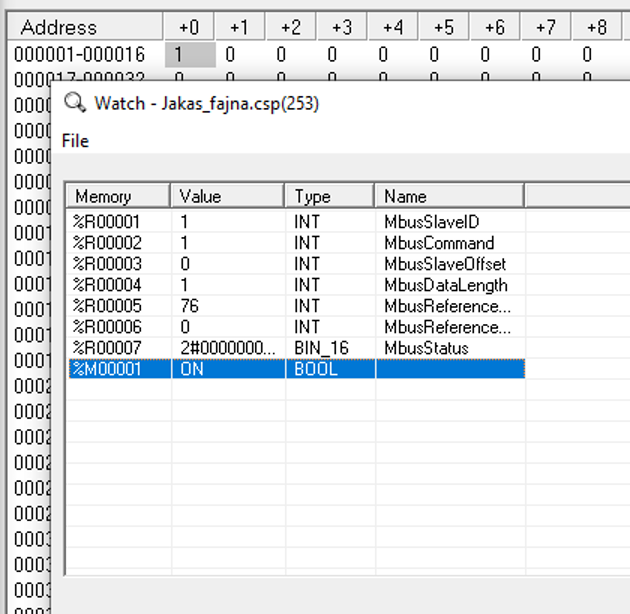
\includegraphics[width=0.5\textwidth]{media/5_test1_3_ONnacewce.png}
    \caption{Rejestry w aplikacji \textit{Cspace} po otrzymaniu sygnału z cewki}
    \label{fig:zdj13}
\end{figure}

\newpage

Na zdjęciu \ref{fig:zdj12} przedstawiona jest ramka komunikacji. Ramka pierwsza (\texttt{Rx}) jest podzielona na dwie linijki. Kod ten jest zapisany w kodzie heksadecymalnym. 

W pierwszej linijce znajduje się zapytanie urządzenia Modbus do PLC. Kolejne bajty oznaczają:
\begin{itemize}
    \item \textbf{Adres Slave'a} - 01
    \item \textbf{Kod funkcji} - 01 (odczyt statusu cewek)
    \item \textbf{Adres początkowy} - 00 00
    \item \textbf{Liczba odczytywanych bajtów} - 00 01
    \item \textbf{Suma kontrolna CRS} - FD CA
\end{itemize}

W trzeciej linijce znajduje się informacja o \textit{Protocol Data Unit} tutaj wynoszącym 256.

W czwartej linijce znajduje się potwierdzenie, że system próbuje odczytać 1 bit od adresu 0.

W ostatniej linijce znajduje się odpowiedź urządzenia Modbus. Kolejne bajty oznaczają:
\begin{itemize}
    \item \textbf{Adres Slave'a} - 01
    \item \textbf{Kod funkcji} - 01 (odczyt statusu cewek)
    \item \textbf{Liczba bajtów} - 00
    \item \textbf{Stan bajtów} - 00
    \item \textbf{Suma kontrolna CRS} - 51 88
\end{itemize}


\begin{figure}[H]
    \centering
    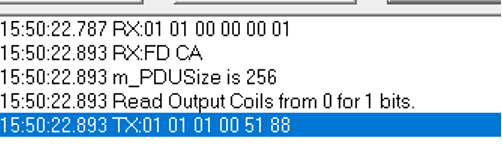
\includegraphics[width=0.5\textwidth]{media/5_test1_2_comszModbusapp.png}
    \caption{Ramki komunikacyjne dla testu 1}
    \label{fig:zdj12}
\end{figure}


\newpage
\subsection{Test 2}
 W teście drugim należało zrobić cykliczne wysyłanie wartości licznika do Slave'a. Aby to otrzymać należało w pierwszej  kolejności stworzyć nową drabinkę, przedstawioną na zdjęciu \ref{fig:zdj14}, za blokiem \textit{CTU} oraz rejestrem \textit{T\_SEC} który tworzy sygnał prostokątny o częstotliwości 1Hz, dzięki czemu licznik CTU zwiększał wartość z taką częstotliwością.

\begin{figure}[H]
    \centering
    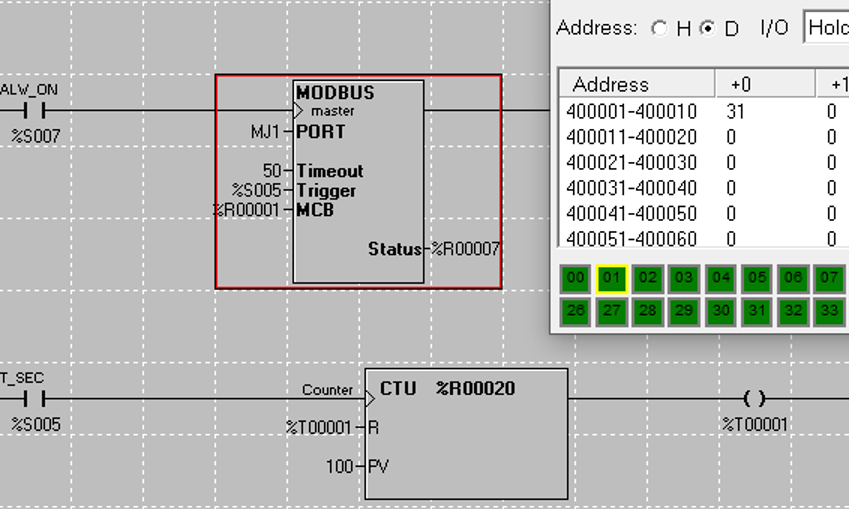
\includegraphics[width=0.5\textwidth]{media/5_test2_1_timer.png}
    \caption{Drabinka z blokiem CTU oraz odczyt licznika w aplikacji \textit{ModRSsim2}} 
    \label{fig:zdj14}
\end{figure}

Ponad to należało zmienić wartości w tagach komunikacyjnych, zgodnie z tabelą \ref{tab:tagi2}, po to aby zmienna automatycznie zapisywała się i mogła być bez problemowo odczytywana w aplikacji \textit{ModRSsim2}. Wartości w tagach komunikacyjnych są takie same jak w teście pierwszym, z wyjątkiem zmiany wartości w tagu\textit{MbusCommand}, \textit{MbusReferenceType} oraz \textit{MbusReferenceOffset}.

\begin{table}[h]
    \caption{Opis tagów komunikacyjnych dla testów 2}
    \begin{tabular}{|l|l|l|}
    \hline    
    \textbf{Adres} & \textbf{Nazwa tagu}  & \textbf{Opis} \\\hline
    R01   & MbusSlaveID = 1  & \makecell{Modbus Function Code = 6 oznacza Write Single Register} \\\hline 
    R02   & MbusCommand = 6 & \makecell{Modbus Function Code = 1 oznacza Read Coils} \\\hline
    R03   & MbusSlaveOffset = 0 & \makecell{Adres cewki  w Slave, którą chcemy odczytać.\\Cewka nr 1 ma adres 0.} \\\hline
    R04   & MbusDataLength = 1 & \makecell{Długość danych, które chcemy odczytać - 1 bit.} \\\hline
    R05   & MbusReferenceType = 8  & \makecell{Typ rejestru, który chcemy zapisać.\\8 oznacza rejestr typu \%R} \\\hline
    R06   & MbusReferenceOffset = 19 & \makecell{Adres rejestru w PLC, którego wartość chcemy zapisać do Slave'a.\\Rejestr R20 ma adres Modbus 19.} \\\hline
    R07   & MbusStatus & \makecell{Rejestr przechowujący wynik działania bloku,\\można z niego odczytać ewentualne błędy komunikacji.} \\\hline
    \end{tabular}
    \label{tab:tagi2}
\end{table}


Na zdjęciu \ref{fig:zdj15} przedstawiona jest ramka komunikacji. Ramka pierwsza (\texttt{Rx}) jest podzielona na dwie linijki. Kod ten jest zapisany w kodzie heksadecymalnym. 

W pierwszej linijce znajduje się zapytanie urządzenia Modbus do PLC. Kolejne bajty oznaczają:
\begin{itemize}
    \item \textbf{Adres Slave'a} - 01
    \item \textbf{Kod funkcji} - 06 (Zapis pojedynczego rejestru)
    \item \textbf{Adres początkowy} - 00 00
    \item \textbf{Liczba odczytywanych bajtów} - 00 50
    \item \textbf{Suma kontrolna CRS} - 89 F6
\end{itemize}


W trzeciej linijce znajduje się informacja o \textit{Protocol Data Unit} tutaj wynoszącym 256.

W czwartej linijce znajduje się potwierdzenie, że system odczytuje 1 rejestr z adresu 0.

W ostatniej linijce znajduje się odpowiedź urządzenia Modbus. Kolejne bajty oznaczają:
\begin{itemize}
    \item \textbf{Adres Slave'a} - 01
    \item \textbf{Kod funkcji} - 06 (zapis pojedynczego rejestru)
    \item \textbf{Adres początkowy} - 00 00 
    \item \textbf{Stan bajtów} - 00 50
    \item \textbf{Suma kontrolna CRS} - 89 F6
\end{itemize}


\begin{figure}[H]
    \centering
    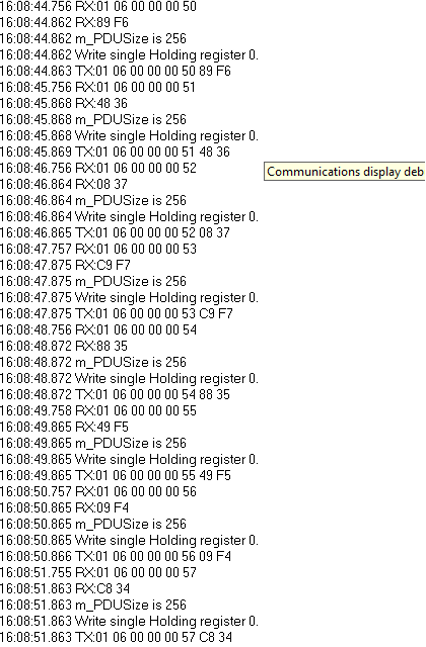
\includegraphics[width=0.5\textwidth]{media/5_test2_2_rejestrzModbusapp.png}
    \caption{Ramki komunikacyjne dla testu 2}
    \label{fig:zdj15}
\end{figure}

\newpage
\section{Zadania}
\subsection{Zadanie 1}
W zadaniu pierwszym należało stworzyć program który miał za zadanie działać analogicznie jak w teście pierwszym, z tą różnicą że zamiast odczytać stan tylko cewki pierwszej to należało odczytać stan 16 cewek zaczynając od cewki 17. Aby to zrobić należało zmienić wartości w tagach komunikacyjnych zgodnie z tabelą \ref{tab:tagi3}.

% \begin{figure}[H]
%     \centering
%     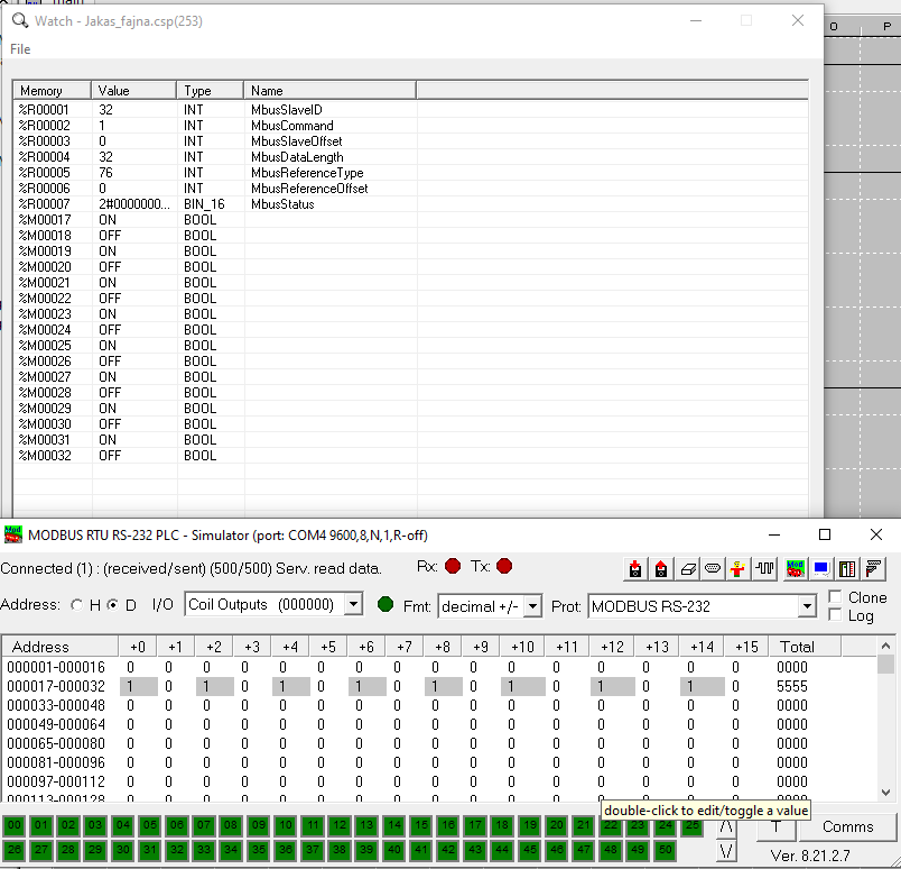
\includegraphics[width=0.5\textwidth]{media/7_1_1_rejestr.png}
%     \caption{Stanowisko laboratoryjne (zdjęcie z konspektu)}
%     \label{fig:zdj16}
% \end{figure}


\begin{table}[h]
    \caption{Opis tagów komunikacyjnych dla zadania 1}
    \begin{tabular}{|l|l|l|}
    \hline    
    \textbf{Adres} & \textbf{Nazwa tagu}  & \textbf{Opis} \\\hline
    R01   & MbusSlaveID = 1  & \makecell{Adres Slave'a odbierającego wiadomość.\\ModRSsim ma adres 1.} \\\hline 
    R02   & MbusCommand = 1 & \makecell{Modbus Function Code = 1 oznacza Read Coils} \\\hline
    R03   & MbusSlaveOffset = 0 & \makecell{Adres cewki  w Slave, którą chcemy odczytać.\\Cewka nr 1 ma adres 0.} \\\hline
    R04   & MbusDataLength = 32 & \makecell{Długość danych, które chcemy odczytać - 32 bit.} \\\hline
    R05   & MbusReferenceType = 76  & \makecell{Typ rejestru, który chcemy odczytać.\\76 oznacza rejestr typu Memory (\%M)} \\\hline
    R06   & MbusReferenceOffset = 0 & \makecell{Adres pamięci w PLC, do którego chcemy zapisać stan cewki,\\czyli adres bitu \%M1.} \\\hline
    R07   & MbusStatus & \makecell{Rejestr przechowujący wynik działania bloku,\\można z niego odczytać ewentualne błędy komunikacji.} \\\hline
    M17 - M32 &  &\makecell{Rejestry, do których zapisywane są stany cewek.\\M17 - M32 odpowiadają cewkom 17 - 32.} \\\hline
    \end{tabular}
    \label{tab:tagi3}
\end{table}

\newpage
Dzięki tak przypisanym tagom możliwe było odczytanie stanu cewek, które były przypisane do rejestrów M17 - M32. Aby to zrobić należało zmienić stan cewek w aplikacji \textit{ModRSsim2}. Aby odczytać stan cewek należało kliknąć przycisk na układzie tak jak na zdjęciu \ref{fig:zdj6}. W momencie kiedy cewka \textit{X} w aplikacji była ustawiona na 1, wartość zmiennej \textit{\%M0000X} zmienił się z \texttt{OFF} na \texttt{ON}.

\begin{figure}[H]
    \centering
    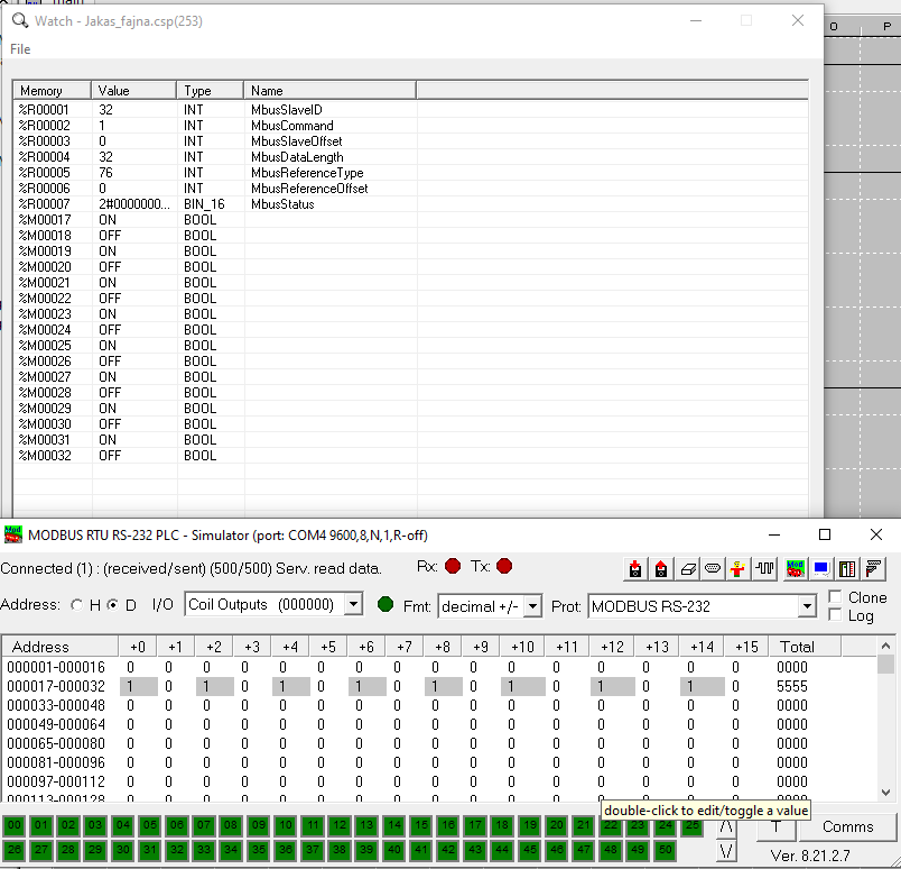
\includegraphics[width=0.5\textwidth]{media/7_1_2_WatchTable.png}
    \caption{Tagi komunikacyjne oraz rejestry dla zadania 1}
    \label{fig:zdj17}
\end{figure}

\newpage
Na zdjęciu \ref{fig:zdj18} przedstawiona jest ramka komunikacji. Ramka pierwsza (\texttt{Rx}) jest podzielona na dwie linijki. Kod ten jest zapisany w kodzie heksadecymalnym. 

W pierwszej linijce znajduje się zapytanie urządzenia Modbus do PLC. Kolejne bajty oznaczają:
\begin{itemize}
    \item \textbf{Adres Slave'a} - 20
    \item \textbf{Kod funkcji} - 01 (odczyt statusu cewek)
    \item \textbf{Adres początkowy} - 00 00
    \item \textbf{Liczba odczytywanych bajtów} - 00 20
    \item \textbf{Suma kontrolna CRS} - 3B 63
\end{itemize}

W trzeciej linijce znajduje się informacja o \textit{Protocol Data Unit} tutaj wynoszącym 256.

W czwartej linijce znajduje się potwierdzenie, że system odczytuje bajty w zakresie od 0 do 32.

W ostatniej linijce znajduje się odpowiedź urządzenia Modbus. Kolejne bajty oznaczają:
\begin{itemize}
    \item \textbf{Adres Slave'a} - 20
    \item \textbf{Kod funkcji} - 01 (odczyt statusu cewek)
    \item \textbf{Liczba bajtów} - 04 
    \item \textbf{Wartość bajtów} - 00 00 55 55
    \item \textbf{Suma kontrolna CRS} - 35 BC
\end{itemize}



\begin{figure}[H]
    \centering
    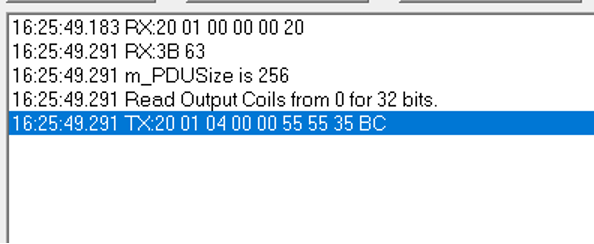
\includegraphics[width=0.5\textwidth]{media/7_1_3_comsy.png}
    \caption{Ramki komunikacyjne dla zadania 1}
    \label{fig:zdj18}
\end{figure}
\newpage
\subsection{Zadanie 2}
W zadaniu drugim należało stworzyć program który miał za zadanie zmieniać wartości cewki Slave'a. Aby to zrobić należało zmienić wartości w tagach komunikacyjnych zgodnie z tabelą \ref{tab:tagi4}. Dzięki tak przypisanym tagom możliwe było zapisanie stanu cewki, która była przypisana do rejestru M1. Aby to zrobić należało zmienić stan cewki w tagach komunikacji. Aby odczytać stan cewki należało kliknąć przycisk na układzie tak jak na zdjęciu \ref{fig:zdj6}. W momencie kiedy cewka \textit{X} w tagach była ustawiona na \texttt{ON}, wartość zmiennej w aplikacji \textit{ModRSsim2} zmienił się z 0 na 1, co przedstawione jest na zdjęciu \ref{fig:zdj19}.

\begin{table}[h]
    \caption{Opis tagów komunikacyjnych dla zadania 2}
    \begin{tabular}{|l|l|l|}
    \hline    
    \textbf{Adres} & \textbf{Nazwa tagu}  & \textbf{Opis} \\\hline
    R01   & MbusSlaveID = 1  & \makecell{Adres Slave'a odbierającego wiadomość.\\ModRSsim ma adres 1.} \\\hline 
    R02   & MbusCommand = 15 & \makecell{Modbus Function Code = 15 oznacza Force Multiple Coils} \\\hline
    R03   & MbusSlaveOffset = 0 & \makecell{Adres cewki  w Slave, którą chcemy nadpisać.\\Cewka nr 1 ma adres 0.} \\\hline
    R04   & MbusDataLength = 5 & \makecell{Długość danych, które chcemy nadpisać - 5 bitów.} \\\hline
    R05   & MbusReferenceType = 76  & \makecell{Typ rejestru, który chcemy odczytać.\\76 oznacza rejestr typu Memory (\%M)} \\\hline
    R06   & MbusReferenceOffset = 0 & \makecell{Adres pamięci w PLC, do którego chcemy zapisać stan rejestru,\\czyli adres bitu \%M1.} \\\hline
    R07   & MbusStatus & \makecell{Rejestr przechowujący wynik działania bloku,\\można z niego odczytać ewentualne błędy komunikacji.} \\\hline
    M1 - M5 &  &\makecell{Rejestry, w których zapisane będą stany cewek.\\M1 - M5 odpowiadają cewkom 1 - 5} \\\hline
    \end{tabular}
    \label{tab:tagi4}
\end{table}


\begin{figure}[H]
    \centering
    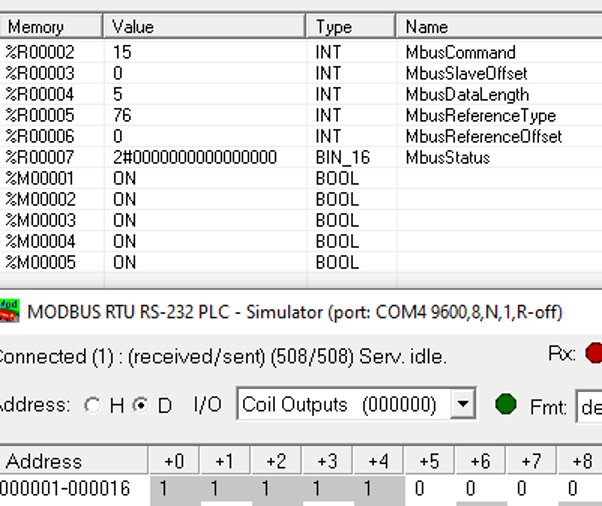
\includegraphics[width=0.5\textwidth]{media/7_2_1_watchtable.png}
    \caption{Tagi komunikacyjne oraz rejestry dla zadania 2}
    \label{fig:zdj19}
\end{figure}

\newpage

Na zdjęciu \ref{fig:zdj20} przedstawiona jest ramka komunikacji. Ramka pierwsza (\texttt{Rx}) jest podzielona na dwie linijki. Kod ten jest zapisany w kodzie heksadecymalnym. 

W pierwszej linijce znajduje się zapytanie urządzenia Modbus do PLC. Kolejne bajty oznaczają:
\begin{itemize}
    \item \textbf{Adres Slave'a} - 20
    \item \textbf{Kod funkcji} - 0F -> 15[dec](przypisanie wartości do wielu cewek)
    \item \textbf{Adres początkowy} - 00 00
    \item \textbf{Liczba odczytywanych bajtów} - 00 05
    \item \textbf{Dane do zapisu} - 1F
    \item \textbf{Suma kontrolna CRS} - FD CA
\end{itemize}

W trzeciej linijce znajduje się informacja o \textit{Protocol Data Unit} tutaj wynoszącym 256.

W czwartej linijce znajduje się potwierdzenie, że system przypisuje wartości do wielu cewek, w zakresie 0 - 5 bitów.

W ostatniej linijce znajduje się odpowiedź urządzenia Modbus. Kolejne bajty oznaczają:
\begin{itemize}
    \item \textbf{Adres Slave'a} - 20
    \item \textbf{Kod funkcji} - 0F - 15[dec](przypisanie wartości do wielu cewek)
    \item \textbf{Adres początkowy} - 00 00 
    \item \textbf{Stan bajtów} - 00 05
    \item \textbf{Suma kontrolna CRS} - 93 79
\end{itemize}


\begin{figure}[H]
    \centering
    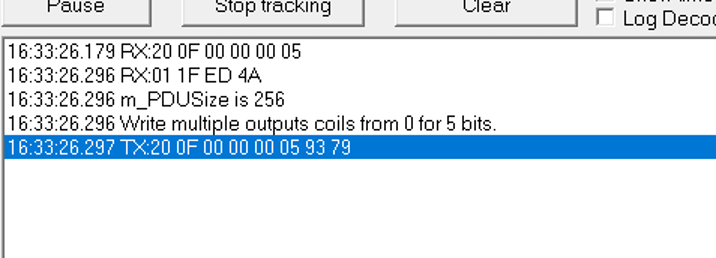
\includegraphics[width=0.5\textwidth]{media/7_2_2_comsy.png}
    \caption{Ramki komunikacyjne dla zadania 2}
    \label{fig:zdj20}
\end{figure}

\newpage
\subsection{Zadanie 3}
W zadaniu trzecim należało zmodyfikować kod tak aby możliwe było zapisanie danych na rejestrze PLC. Aby to zrobić należało ustawić tagi zgodnie z tabelą \ref{tab:tagi5}, dodatkowo należało pamiętać aby typ zmiennych przy rejestrach w których zapisywane były dane były typu \textit{INT}, a dane były zapisywane zgodnie z kodem ASCI. Dzięki czemu możliwe było odczytanie w aplikacji tekstu, co przedstawione jest na zdjęciu \ref{fig:zdj21}.


\begin{table}[h]
    \caption{Opis tagów komunikacyjnych dla zadania 3}
    \begin{tabular}{|l|l|l|}
    \hline    
    \textbf{Adres} & \textbf{Nazwa tagu}  & \textbf{Opis} \\\hline
    R01   & MbusSlaveID = 1  & \makecell{Adres Slave'a odbierającego wiadomość.\\ModRSsim ma adres 1.} \\\hline 
    R02   & MbusCommand = 16 & \makecell{Modbus Function Code = 16 oznacza Preset Multiple Register} \\\hline
    R03   & MbusSlaveOffset = 0 & \makecell{Adres cewki w Slave, którą chcemy nadpisać.\\Cewka nr 1 ma adres 0.} \\\hline
    R04   & MbusDataLength = 3 & \makecell{Długość danych, które chcemy nadpisać - 3 bity.} \\\hline
    R05   & MbusReferenceType = 8  & \makecell{Typ rejestru, który chcemy odczytać.\\8 oznacza rejestr typu Register (\%R)} \\\hline
    R06   & MbusReferenceOffset = 7 & \makecell{Adres rejestru w PLC, do którego chcemy zapisać zmienną,\\czyli adres \%R8.} \\\hline
    R07   & MbusStatus & \makecell{Rejestr przechowujący wynik działania bloku,\\można z niego odczytać ewentualne błędy komunikacji.} \\\hline
    R8 - R10 &  &\makecell{Rejestry, w które wpisywane będą litery \texttt{AGH}.\\R8 - R10 odpowiadają rejestrom od 8 do 10.} \\\hline
    \end{tabular}
    \label{tab:tagi5}
\end{table}


\begin{figure}[H]
    \centering
    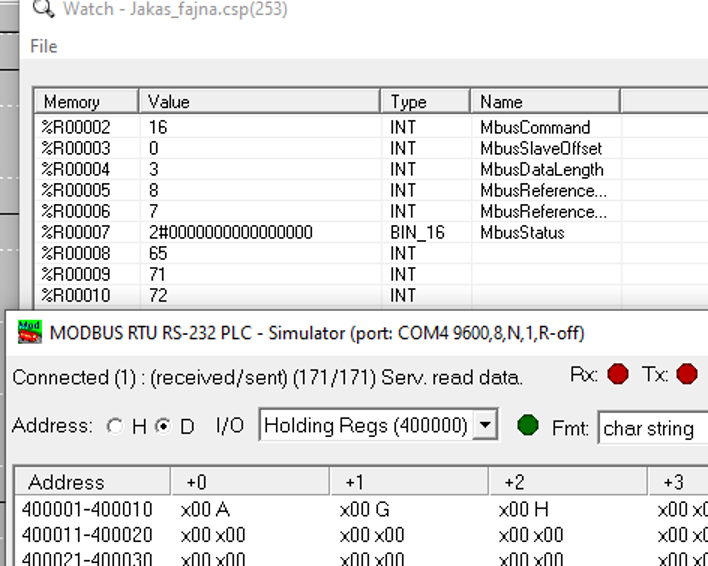
\includegraphics[width=0.5\textwidth]{media/7_3_1_napis.png}
    \caption{Tagi komunikacyjne oraz rejestry dla zadania 3}
    \label{fig:zdj21}
\end{figure}

\newpage

Na zdjęciu \ref{fig:zdj22} przedstawiona jest ramka komunikacji. Ramka pierwsza (\texttt{Rx}) jest podzielona na dwie linijki. Kod ten jest zapisany w kodzie heksadecymalnym. 

W pierwszej linijce znajduje się zapytanie urządzenia Modbus do PLC. Kolejne bajty oznaczają:
\begin{itemize}
    \item \textbf{Adres Slave'a} - 01
    \item \textbf{Kod funkcji} - 10 - > 16[dec](Zapis wielu rejestrów)
    \item \textbf{Adres początkowy} - 00 00
    \item \textbf{Liczba rejestrów do zapisu} - 00 03
    \item \textbf{Dane do rejestru} - 00 41 00 47 00 48
    \item \textbf{Suma kontrolna CRS} - 6A AC
\end{itemize}

W trzeciej linijce znajduje się informacja o \textit{Protocol Data Unit} tutaj wynoszącym 256.

W czwartej linijce znajduje się potwierdzenie, że system zapisuje dane do rejestrów w zakresie 0 do 3.

W ostatniej linijce znajduje się odpowiedź urządzenia Modbus. Kolejne bajty oznaczają:
\begin{itemize}
    \item \textbf{Adres Slave'a} - 01
    \item \textbf{Kod funkcji} - 10 -> 16 (Zapis wielu rejestrów)
    \item \textbf{Adres początkowy} - 00 00
    \item \textbf{Liczba zapisanych rejestrów} - 00 03
    \item \textbf{Suma kontrolna CRS} - 80 08
\end{itemize}



\begin{figure}[H]
    \centering
    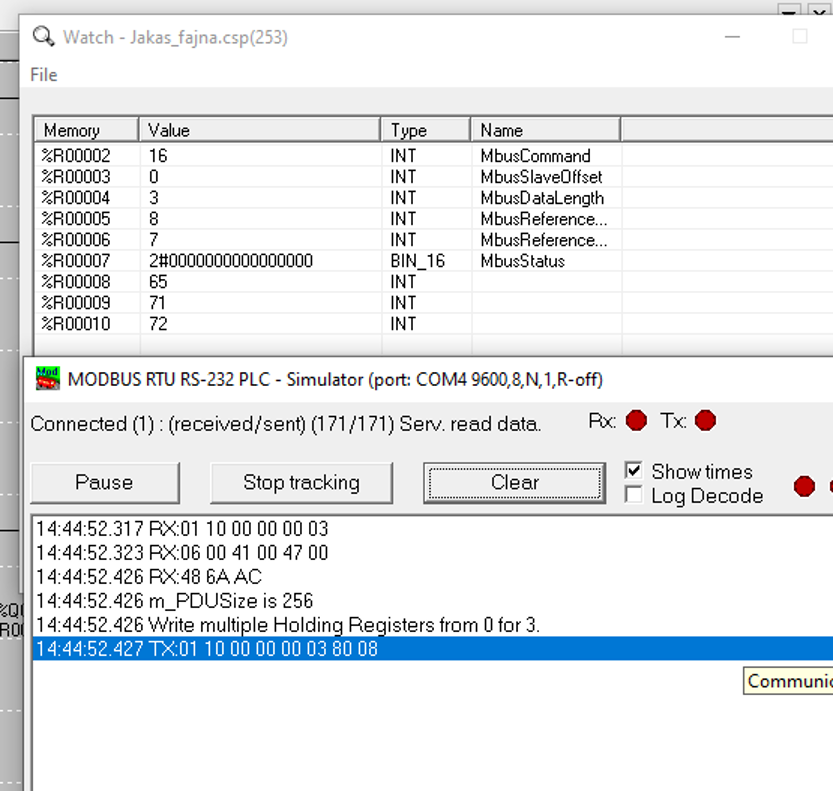
\includegraphics[width=0.5\textwidth]{media/7_3_2_comsy.png}
    \caption{Ramki komunikacyjne dla zadania 3}
    \label{fig:zdj22}
\end{figure}

\newpage
\subsection{Zadanie 4}
W zadaniu ostatnim należało edytować tagi komunikacyjne tak aby na \textit{\%R07} pojawił się błąd. W wypadku gdy nie wystąpi żaden błąd ma on wartość 1, czyli wszystkie bity poza najmniej znaczącym mają wartość 0.

Na zdjęciu \ref{fig:zdj24} przedstawiony jest błąd wynikający z próby przesłania zbyt dużej liczby danych. Widać że na tagu \textit{\%R07} zamiast zmienić się pierwszy bit, zmienią się bity 2 oraz 6, co zgodnie z dokumentacją oznacza \textit{Request Failed} oraz \textit{MCB - Invalid I/O Reference}. Na zdjęciu widać również że w aplikacji \textit{ModRSsim2} w comsach nie pojawia się żadna informacja co oznacza że już na poziomie Modbusa sygnał jest zatrzymywany.

Natomiast na zdjęciu \ref{fig:zdj23} przedstawia błąd wynikający z próby wywołania błędnej funkcji, co również możemy odczytać z kodu zapisanego w \textit{\%R07}. W tym przypadku zmienia się bit 2, który jak poprzednio oznacza \textit{Request Failed} oraz bit 5, który oznacza \textit{Invalid Function}. W tym przypadku również żadna informacja nie pojawia się w aplikacji \textit{ModRSsim2}.



\begin{figure}[!ht]
    \centering
        % Pod figura 1
        \subfloat[Błąd 'Invalid I/O Reference']{    
            \centering
            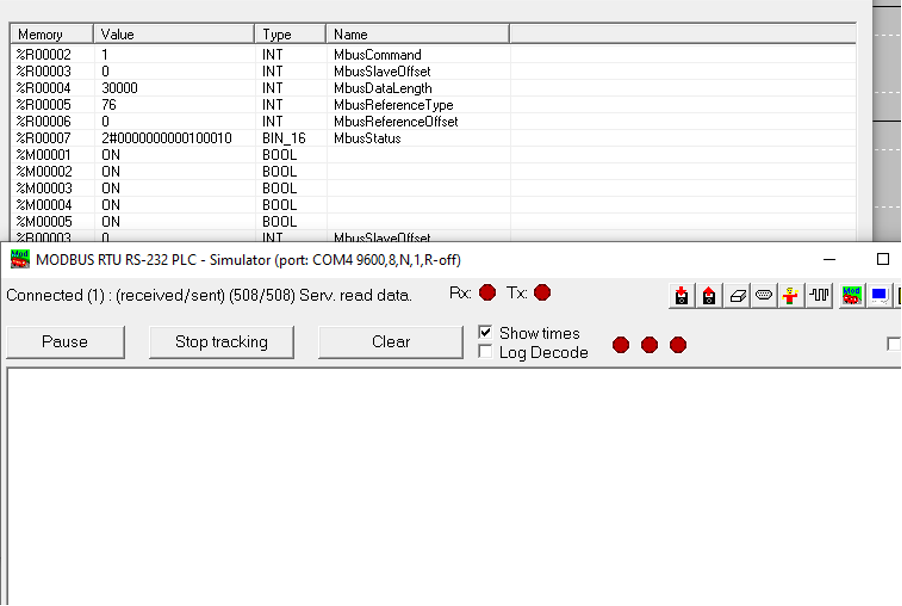
\includegraphics[width=0.45\textwidth]{media/7_4_2_niepoprawnyzakresdanych.png}
            \label{fig:zdj24}}
        % Pod figura 2
        \subfloat[Debugowanie aktywnego układu]{
            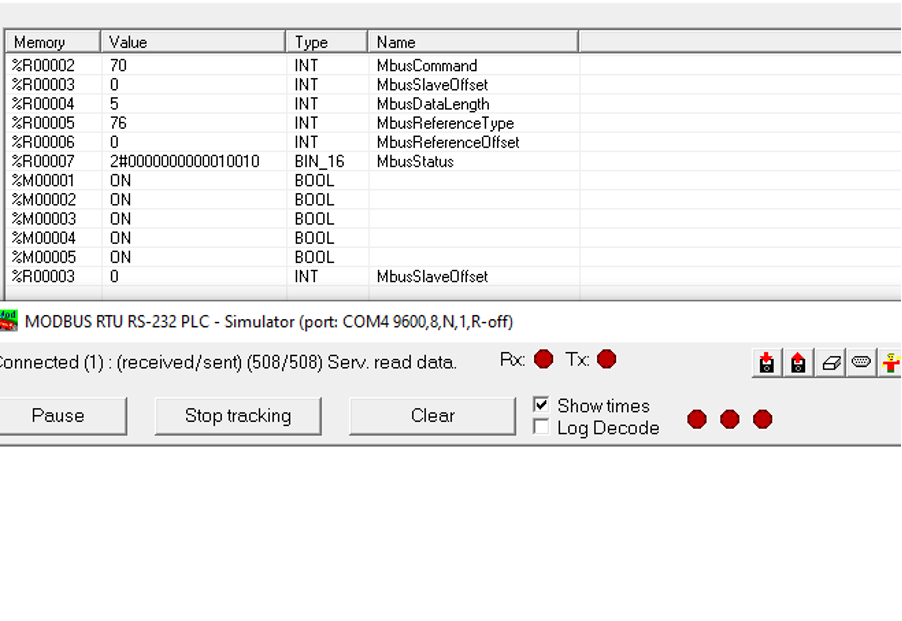
\includegraphics[width=0.45\textwidth]{media/7_4_1_niepoprawnykod.png}       
             \label{fig:zdj23}
        }
    \caption{Błędne tagi komunikacyjne}
    \label{fig:main2}
\end{figure}
\newpage
\section{Podsumowanie}
Na zajęciach należało zapoznać się z obsługą protokołu Modbus oraz z aplikacją \textit{ModRSsim2}. Komunikacja ta jest jedną z najpopularniejszych komunikacji w przemyśle.

Jedną z najważniejszych umiejętności do obsługi tej komunikacji jest umiejętność odczytu ramek oraz znajomość kodów komunikatów co należało wykonać w zadaniach. Dzięki temu można było nauczyć się jak działa komunikacja oraz jak można ją wykorzystać w praktyce. W zadaniach należało zapoznać się z kodami do obsługi modbusa oraz nauczyć się jak w różny sposób można przesyłać dane. Ponadto należało również zapoznać się z tagiem \textit{MbusStatus} co jest niezbędną umiejętnością w obsłudze urządzeń.

Ćwiczenia te umożliwiły zapoznanie się z podstawami działania protokołu Modbus oraz lepsze zrozumienie jego mechanizmów.

\end{document}
